\chapter{Was sind Workflows?}  % Kapitel % Steht dann über dem Text
\label{chapter:Was sind Workflows?}  % Steht als Text im Inhaltsverzeichnis
\index{Was sind Workflows?} % für das Stichwortverzeichnis

\textbf{Allgmeine Definition:}\\
Ein Workflow bildet die an einem Arbeitsprozess beteiligten Personen und Arbeitsprozesse in einem Prozessmodell ab. Workflow-Management beabsichtigt betriebsinterne Ressourcen und Tätigkeiten der Mitarbeiter innerhalb eines Geschäftsprozesses nach festen Parametern zu strukturieren, zu operationalisieren und zu optimieren.\\
\\
\textbf{Workflows bei CodeRed:}\\
Als Workflows werden alle Arbeitsabläufe sowie Prozesse über ein Ticket, im CodeRed System festgehalten. Unter jedem Ticket gibt es den Workflow Bereich. Um einen neuen Workflow anzulegen muss nur auf den Link geklickt werden. Danach wird die individuelle Workflow Unternavigation geladen. \\
\\
\begin{figure}[h!]
\begin{center}
   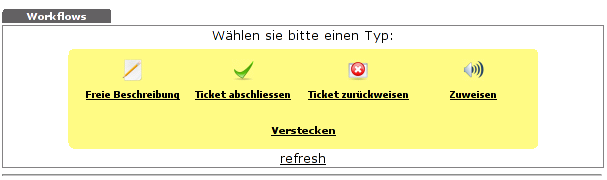
\includegraphics[width=400pt]{../bilder/workflow_navi_neu.png}
   \caption{Workflow Navigation}
   \label{Workflow Navigation}
\end{center}
\end{figure}
Welche Möglichkeiten ein User im Workflowbereich hat wird durch seine zugewiesen Rechte im System und an dem jeweiligen Ticket bestimmt. Wenn zum Beispiel ein Betreuer nicht einem Ticket zugewiesen ist, kann er zwar ein Workflow erstellen um seinem Kollegen mit einem Tipp zu Helfen, er kann das Ticket aber nicht Abschließen.\\
\newpage
Leider werden die Workflows ab aufrufen der Ticket nicht direkt mit geladen, deswegen muss um die Workflow anzeigen zu lassen auf den Refresh Link geklickt werden. Nach dem Klicken werden im Unterenbereich die vorhanden Workflows zu einem Ticket geladen.\\
\begin{figure}[h!]
\begin{center}
   \includegraphics[width=450pt]{../bilder/Workflow_all.png}
   \caption{Workflows}
   \label{Workflows}
\end{center}
\end{figure}
\newpage
Jedes Ticket hat einen eigenen Workflowbereich der mit dem Zuweisen des Tickets beginnt und mit dem Abschließen endet.\\
\\
\begin{figure}[h!]
\begin{center}
   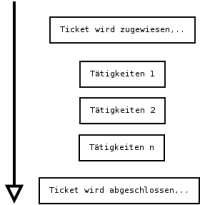
\includegraphics[width=200pt]{../bilder/workflow_erz.png}
   \caption{Workflows}
   \label{Workflows}
\end{center}
\end{figure}
\begin{figure}[htbp!]
\begin{center}
   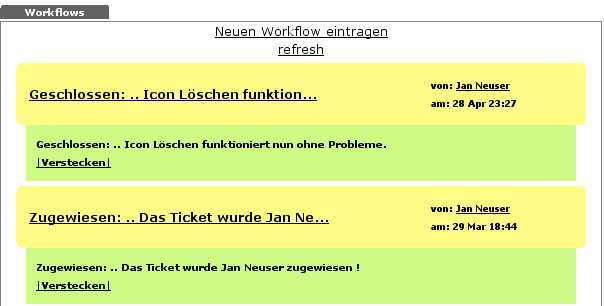
\includegraphics[width=400pt]{../bilder/workflow_auf.png}
   \caption{Workflows}
   \label{Workflows}
\end{center}
\end{figure}
\\
Jeder Workflow ist zuerst nur mit der Überschrift und den Erstellerdaten zu sehen. Mit einem Klick auf die Überschrift, wird der Vollständige Workflow angezeigt. Um die Übersichtlichkeit zu bewahren, können diese Texte mit einem Klick wieder versteckt werden.
 
